\documentclass{article} % For LaTeX2e
\usepackage{nips14submit_e,times}
\usepackage{hyperref}
\usepackage{url}
\usepackage{amsmath,amsfonts,amsthm}
\usepackage{bbm}
\usepackage{algorithm,algorithmic}
\usepackage{graphicx}
\usepackage{bm}
\usepackage{bbm}
\usepackage[titletoc]{appendix}
\usepackage{wrapfig}
\usepackage{afterpage}
\usepackage{amssymb}
\usepackage{booktabs}
\usepackage{ulem}
\usepackage{multirow}

\def\B#1{\bm{#1}}
%\def\B#1{\mathbf{#1}}
\def\trans{\mathsf{T}}

%\renewcommand{\labelitemi}{--}

\newtheorem{theorem}{Theorem} \newtheorem{lemma}[theorem]{Lemma}
\newtheorem{proposition}[theorem]{Proposition}
\newtheorem{corollary}[theorem]{Corollary}
\newtheorem{definition}[theorem]{Definition}
\newtheorem{remark}{Remark}

%%%%%%%%%%%%%%%%%%%%%%%%%%%%%%%%%%%%%%%%%%%%%%%%%%%%%%%%%%%%%%%%%%%%%%%%%%%%%%%

\title{Semi-Supervised Factored Logistic Regression for
High-Dimensional Neuroimaging Data}

\newcommand{\fix}{\marginpar{FIX}}
\newcommand{\new}{\marginpar{NEW}}
\DeclareMathOperator{\proj}{proj}
\DeclareMathOperator{\softmax}{softmax}
\DeclareMathOperator{\prox}{prox}
\DeclareMathOperator{\Prox}{Prox}
\DeclareMathOperator{\im}{im}

% macros from michael's .tex
\DeclareMathOperator{\dist}{dist} % The distance.
\DeclareMathOperator{\argmin}{argmin}
\DeclareMathOperator{\argmax}{argmax}
\DeclareMathOperator{\Id}{Id}
\DeclareMathOperator{\abs}{abs}
\newcommand{\R}{\mathbb{R}}
\newcommand{\N}{\mathbb{N}}
\newtheorem{thm}{Theorem}[section]
\newtheorem{prop}[thm]{Proposition}
\newtheorem{lem}[thm]{Lemma}
\newtheorem{cor}[thm]{Corollary}


\newcommand{\suggestadd}[1]{{\color{blue} #1}}
\newcommand{\suggestremove}[1]{{\color{red} \sout{#1}}}

%\nipsfinalcopy % Uncomment for camera-ready version
\nipsfinalfalse
%%%%%%%%%%%%%%%%%%%%%%%%%%%%%%%%%%%%%%%%%%%%%%%%%%%%%%%%%%%%%%%%%%%%%%%%%%%%%%%

\begin{document}

\author{Danilo Bzdok, Michael Eickenberg, Olivier Grisel,
  Bertrand Thirion,
  Ga\"el Varoquaux \\\textbf{\textit{email:} }firstname.lastname@inria.fr}

\maketitle

\begin{abstract}
Imaging neuroscience links human behavior to aspects of brain
biology in ever-increasing datasets.
%
Existing neuroimaging methods typically perform either discovery of unknown
neural structure or testing of neural structure associated with mental tasks.
%
However, testing hypotheses on the neural correlates of
larger mental task sets
necessitates adequate representations for the observations.
%
We therefore propose to blend
representation modelling and task classification into
a unified statistical learning problem.
%
A multinomial logistic regression is introduced that is
constrained by factored coefficients and coupled with an autoencoder.
%
We show that this approach yields more accurate and interpretable
neural models of psychological tasks in a reference dataset,
as well as better generalization to other datasets.
%

% OUR keywords
%\textbf{\\keywords}: curse of dimensionality; semi-supervised learning;
%fMRI; systems neuroscience

% official NIPS keywords
\textbf{\\keywords}: Brain Imaging, Cognitive Science, Semi-Supervised Learning, Systems Biology

\end{abstract}

\section{Introduction}
%
Methods for neuroimaging research can be grouped by discovering
neurobiological structure or assessing the neural correlates associated
with mental tasks.
To \textit{discover}, on the one hand,
spatial distributions of neural activity
structure across time,
independent component analysis (ICA) is often used
\cite{beckmann2005}.
It decomposes the BOLD (blood-oxygen level-dependent) signals into the
primary modes of variation.
The ensuing spatial activity patterns are believed to represent
brain networks of
functionally interacting regions \cite{smith2009}.
Similarly, sparse principal component analysis (SPCA)
has been used to
separate BOLD signals into parsimonious network components
\cite{varoqu2011}.
The extracted brain networks are probably
manifestations of electrophysiological oscillation frequencies \cite{hipp15}.
Their fundamental organizational role is further
attested by continued covariation during sleep and anesthesia \cite{fox07}.
%
Network discovery by applying ICA or SPCA is typically performed on
task-unrelated (i.e., \textit{unlabeled}) ``resting-state'' data.
These capture brain dynamics
during ongoing random thought without controlled environmental stimulation.
In fact, a large portion of the BOLD signal variation
is known
not to correlate with a particular behavior, stimulus, or experimental task
\cite{fox07}. 

To \textit{test}, on the other hand,
the neural correlates underlying mental tasks,
the general linear model (GLM) is the dominant approach \cite{friston94}.
The contribution of
individual brain voxels is estimated
according to a design matrix of experimental tasks.
Alternatively, psychophysiological interactions (PPI)
elucidate the influence of one brain region on another conditioned
by experimental tasks \cite{friston97}.
As a last example, an increasing number of
neuroimaging studies model
experimental tasks by training classification algorithms on brain signals
\cite{poldrack09decoding}.
All these methods are applied to task-associated (i.e., \textit{labeled})
data that capture brain dynamics
during stimulus-guided behavior.
Two important conclusions can be drawn.
First, the mentioned supervised neuroimaging analyses typically yield
results in a voxel space.
This ignores the fact that the BOLD
signal exhibits spatially distributed patterns
of coherent neural activity.
%
Second, existing supervised neuroimaging analyses
cannot exploit the abundance
of easily acquired resting-state data \cite{biswaldiscovery}.
These may allow better discovery of
the manifold of brain states
due to the high task-rest similarities of neural activity patterns,
as observed using ICA \cite{smith2009}.
% XXX: you don't discuss the absence of information sharing across tasks / cognitions, i.e. the multi-task aspect of your work.

Both these neurobiological properties can be conjointly exploited in an
approach that is
\textit{mixed} (i.e., using rest and task data),
\textit{factored} (i.e., performing network decomposition), and
\textit{multi-task} (i.e., capitalize on neural representations shared across
mental operations).
%
The integration of brain-network discovery into
supervised classification can yield a semi-supervised learning
framework. The most relevant
neurobiological structure should hence be identified
for the prediction problem at hand.
%
Autoencoders suggest themselves because they can emulate
variants of most unsupervised learning algorithms,
including PCA, SPCA, and ICA \cite{hinton06}.
\begin{wrapfigure}{r}{0.40\textwidth}
  \centering
  %\captionsetup{labelformat=nonumber}
    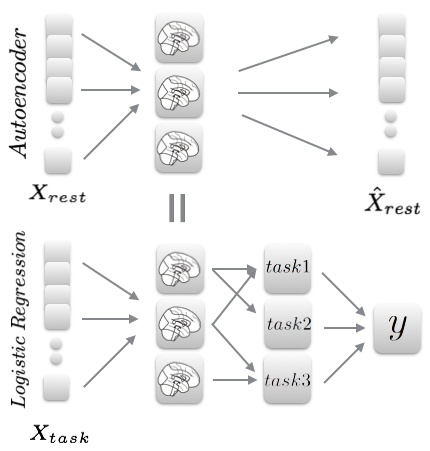
\includegraphics[width=0.40\textwidth]{figures/figure1.png}
  \vspace{-0.7cm}
  \caption {\textbf{Model architecture.}
  Linear autoencoders find an optimized compression of 79,941 brain voxels
  into $n$ unknown activity patterns by improving reconstruction from them.
  The decomposition matrix equates with the bottleneck of
  a factored logistic regression.
  Supervised multi-class learning on task data ($X_{task}$)
  can thus be guided by
  unsupervised decomposition of rest data ($X_{rest}$).
  }
\end{wrapfigure}
%
Autoencoders (AE)
are layered learning models
that condense the input data to
local and global 
representations
via reconstruction under compression prior.
%
% XXX Michael: In fact, they behave like a non-centered PCA, 
% XXX which amounts to just doing an SVD
% XXX which btw is NOT a convex optimization problem, although easy to 
% XXX calculate and with a global optimum.
% XXX Autoencoders are also not one-layered by default. Let's make sure that
% XXX we don't trip up by getting the technicalities wrong and getting 
% XXX reviewers annoyed at us because of it.
% DanilO: cool thanks. That is the stuff, we need.
They behave like a (truncated) PCA
in case of one linear hidden layer and a squared error loss
\cite{baldi1989neural}.
% This architecture yields an optimization objective
% with unique global minimum.
Autoencoders behave like a SPCA if shrinkage terms are added to the
model weights in the optimization objective.
Moreover, they have the characteristics of an ICA in case of tied weights
and adding a nonlinear convex function
at the first layer \cite{le2011ica}.
% XXX What convex transformation? Why is that relevant? Convexity is only
% XXX relevant for the loss
% Danilo: it's about adding a neural-network-like nonconvex function for
% first-layer activation
These authors further demonstrated that ICA, sparse autoencoders, and 
sparse coding are mathematically equivalent
under mild conditions.
%
Thus, autoencoders may flexibly project the neuroimaging data
onto the main directions of variation.

In the present investigation,
a linear autoencoder will be fit to
(unlabeled) rest data and
integrated as a rank-reducing bottleneck
into a multinomial
logistic regression fit to
(labeled) task data.
We can then solve the unsupervised data representation and the
supervised classification, previously studied in isolation,
in an identical statistical learning problem.
%
From the perspective of dictionary learning, the first layer represents
% XXX Michael: This is the crucial difference: The first layer is an analysis
% XXX operation: it extracts information in some way. It may be extracting
% XXX activations for basis functions, in which case it would be the pseudo-
% XXX inverse of those basis functions. But unless they are orthogonal, these
% XXX weights definitely don't represent basis functions themselves. It is 
% XXX the second layer of the autoencoder that represents basis functions. If
% XXX weights are tied, they are one and the same thing, with interesting
% XXX implications. But in general, only the second layer represents a basis.
projectors to the discovered set of basis functions
which are linearly combined 
by the second layer to perform predictions \cite{olshausen96}.
% XXX Michael: ^ This needs to be changed around: This first layer obtains
% XXX activations, the second layer weights are basis functions which are
% XXX multiplied to these activations
%
Neurobiologically, this allows 
delineating a low-dimensional manifold
of brain network patterns and then 
distinguishing mental tasks
by their most discriminative linear combinations.
%
Theoretically, a reduction in model variance should be achieved by
resting-state autoencoders that
privilege the most neurobiologically
valid models in the hypothesis set.
%
Practically, neuroimaging research is frequently suffering from
data scarcity. This limits the set of representations that can be
extracted from GLM analyses based on few participants.
%
We therefore contribute a computational framework that
1) analyzes many problems simultaneously
(thus finds shared representations by ``multi-task learning'')
and
2) exploits unlabeled data,
as they span a space of meaningful configurations.

\section{Methods}
%
\paragraph{Data.}
As the currently biggest openly-accessible reference dataset,
we chose resources from the Human Connectome Project (HCP)
\cite{barch2013}.
Neuroimaging task data with labels of ongoing cognitive processes
were drawn from 500 unrelated,
healthy HCP participants (cf. Appendix for details on datasets).
18 HCP tasks 
were selected that are known to elicit reliable neural activity
across participants (Table \ref{table_tasks}).
In sum, the HCP task data incorporated 8650 first-level activity maps
from 18 diverse paradigms administered to 498 participants (2 removed
due to incomplete data).
All maps were resampled to a common $60\times72\times60$ space of
3mm isotropic voxels and gray-matter masked (at least 10\% tissue
probability).
The supervised analyses were based on labeled HCP task maps with
79,941 voxels of interest representing z-values in gray matter.

\begin{table}[h]
  \resizebox{0.98\textwidth}{!}{%
  \begin{tabular}{l|l|l}
    \hline
  {\bf Cognitive Task} & {\bf Stimuli}                         & {\bf Instruction for participants}                                                \\ \hline
  1 Reward             & \multirow{2}{*}{Card game}            & \multirow{2}{*}{Guess the number of a mystery card for gain/loss of money}        \\ \cline{1-1}
  2 Punish             &                                       &                                                                                   \\ \hline
  3 Shapes             & Shape pictures                        & Decide which of two shapes matches another shape geometrically                    \\ \hline
  4 Faces              & Face pictures                         & Decide which of two faces matches another face emotionally                        \\ \hline
  5 Random             & \multirow{2}{*}{Videos with objects}  & \multirow{2}{*}{Decide whether the circles, squares, triangles act intentionally} \\ \cline{1-1}
  6 Theory of mind     &                                       &                                                                                   \\ \hline
  7 Mathematics        & Spoken numbers                        & Complete addition and subtraction problems                                        \\ \hline
  8 Language           & Auditory stories                      & Choose answer about the topic of the story                                        \\ \hline
  9 Tongue movement    & \multirow{3}{*}{Visual cues}          & Move tongue                                                                       \\ \cline{1-1} \cline{3-3} 
  10 Food movement     &                                       & Squeezing of the left of right toe                                                \\ \cline{1-1} \cline{3-3} 
  11 Hand movement     &                                       & Tapping of the left or right finger                                               \\ \hline
  12 Matching          & \multirow{2}{*}{Shapes with textures} & Decide whether two objects match in shape or texture                             \\ \cline{1-1} \cline{3-3} 
  13 Relations         &                                       & Decide whether object pairs differ both along either shape or texture             \\ \hline
  14 View Bodies       & Pictures                              & Passive watching                                                                   \\ \hline
  15 View Faces        & Pictures                              & Passive watching                                                                   \\ \hline
  16 View Places       & Pictures                              & Passive watching                                                                   \\ \hline
  17 View Tools        & Pictures                              & Passive watching                                                                   \\ \hline
  18 Two-Back          & Various pictures                      & Indicate whether current stimulus is the same as two items earlier                \\ \hline
  \end{tabular}
}
\vspace{-0.2cm}
\caption{\textbf{Description of psychological tasks to predict.}}
\label{table_tasks}
\end{table}

These labeled data were complemented by unlabeled activity maps
from HCP acquisitions of unconstrained resting-state activity
\cite{smith2013resting}.
These reflect brain activity in the absence of controlled thought.
In sum, the HCP rest data concatenated
8000 unlabeled, noise-cleaned rest maps with
40 brain maps from each of 200 randomly selected participants.

We were further interested in the utility of the
optimized low-rank projection
in one task dataset for dimensionality reduction in another task dataset.
To this end, the HCP-derived network decompositions were used as preliminary
step in the classification problem of another large sample.
The ARCHI dataset \cite{pinel07} provides activity maps from
diverse experimental tasks, including auditory and visual perception, motor action,
reading, language comprehension and mental calculation.
Analogous to HCP data, the second task dataset incorporated 1404
labeled, grey-matter masked, and z-scored activity maps
from 18 diverse tasks acquired in 78 participants.

The labeled and unlabeled data were fed into a linear statistical model
composed of an autoencoder and dimensionality-reducing logistic regression.

\paragraph{Linear autoencoder.}
The affine autoencoder takes the input 
$\mathbf{x}$ and projects it into a coordinate system of
latent representations $\mathbf{z}$
and reconstructs it back to $\mathbf{x'}$ by
\begin{eqnarray}
    \mathbf{z} = \mathbf{W_0} \mathbf{x} + \mathbf{b_0} \hspace{2cm}
    \mathbf{x'} = \mathbf{W_1} \mathbf{z} + \mathbf{b_1},
  \label{eq:autoenc}
\end{eqnarray}

where $\mathbf{x \in \mathbb{R}^{d}}$ denotes the vector of $d=79{,}941$
voxel values from each
rest map,
$\mathbf{z \in \mathbb{R}^{n}}$ is the $n$-dimensional hidden state
(i.e., distributed neural activity patterns), and 
$\mathbf{x' \in \mathbb{R}^{d}}$
is the reconstruction vector of the original activity map
from the hidden variables. 
% XXX use bold letters for vectors and matrices
Further, $\mathbf{W_0}$ denotes the weight matrix that
transforms
from input space into the hidden space (encoder),
$\mathbf{W_1}$ is the weight matrix for back-projection
from the hidden variables to the
output space (decoder).
$\mathbf{b_0}$ and $\mathbf{b_1}$ are corresponding bias vectors.
The model parameters $\mathbf{W_0, b_0, b_1}$ are found by
minimizing the expected squared reconstruction error
\begin{equation}
  \mathbb E\left[{\mathcal{L_{AE}}}(\mathbf{x})\right] = %
  \mathbb E\left[\| \mathbf{x} - \mathbf{W_1}(\mathbf{W_0}\mathbf{x} + \mathbf{b_0}) + \mathbf{b_1}) \|^2\right].
\end{equation}

%with \(f_{AE}(\mathbf x) = %
%\mathbf{W_1}(\mathbf{W_0}\mathbf{x} + \mathbf{b_0}) + \mathbf{b_1}\)
% the autoencoder.
% XXX Michael: I don't know to what extent the following makes sense or is
% XXX correct, so I am commenting it
% XXX Danilo: I found this in Bengio's papers somewhere
This reconstruction error criterion equates with
maximizing a lower bound on the mutual information between
input and the learned representation.
% XXX Give a ref ?
Here we choose $\mathbf{W_0}$ and $\mathbf{W_1}$ to be tied, i.e.
$\mathbf{W_0} = \mathbf{W_1^T}$. In particular, this means that the weights
learned are forced to take a two-fold function: That of signal 
\textit{analysis} and that of signal \textit{synthesis}.
The first layer \textit{analyzes}
the data to obtain the cleanest latent representation,
while the second
layer represents building blocks from which to \textit{synthesize} the data
using the latent activations.
Tying these processes together makes the analysis
layer interpretable and pulls all non-zero singular values towards 1. 
Nonlinearities were not applied to the
activations in the first layer.

\paragraph{Factored logistic regression.}
Lossy compression by a low-dimensional bottleneck
is also imposed by the first layer of the factored
multinomial logistic regression.
It gives the probability of an input $\mathbf{x}$ to belong
to a class $i \in \{1, \dots, l\}$
\begin{equation}
  \begin{split}
    P(Y=i|\mathbf{x; V_0,V_1,c_0, c_1}) &= \softmax_i(f_\mathcal{LR}(\mathbf x)),
  \end{split}
  \label{eq:lr}
\end{equation}
where \(f_\mathcal{LR}(\mathbf x) = \mathbf{V_1 (V_0 x + c_0) + c_1}\) computes 
multinomial logits and \(\softmax_i(x) = \exp(x_i)/\sum_j\exp(x_j)\).
The matrix $\mathbf{V_0 \in \mathbb{R}^{dxn}}$
transforms the input $\mathbf{x \in \mathbb{R}^{d}}$
into $n$ latent components
and the matrix $\mathbf{V_1 \in \mathbb{R}^{nxl}}$
projects the latent components
onto hyperplanes that reflect $l$ label probabilities.
$\mathbf{c_0}$ and $\mathbf{c_1}$ are
bias vectors.
The loss function is given by
\begin{equation}
    \mathbb E\left[{\mathcal{L_{LR}}}(\mathbf{x, y})\right] \approx %
\frac{1}{N_{X_{task}}} \sum_{k=0}^{N_{X_{task}}} \log(P(Y=y^{(k)}|\mathbf{x^{(k)}; V_0, V_1, c_0, c_1}).
\label{eq:lr_loss}
\end{equation}

\paragraph{Layer combination.}
Importantly, the optimization problem of the linear autoencoder
and the factored logistic regression
are linked on two levels. First, their transformation matrices mapping from
input to the latent space are tied
\begin{eqnarray}
  \mathbf{V_0} = \mathbf{W_0}.
\end{eqnarray}
We thus search for a compression of the 79,941 voxel values into $n$ latent
components that represent a latent code optimized for both
rest and task activity data.
Second, the objectives of the autoencoder and the factored
logistic regression are interpolated in the common loss function
% XXX Michael: In resolving conflict I opted for my change. Feel free to revert if that was intended.
\begin{equation}
{\mathcal{L}}(\theta, \lambda) = \lambda {\mathcal{L_{LR}}}
+ (1-\lambda)\frac{1}{N_{X_{rest}}} {\mathcal{L_{AE}}} + \Omega(\theta).
  \label{eq:loss_equ}
\end{equation}

In so doing, we search for the combined model parameters
$\theta=\{\mathbf{V_0,V_1,c_0, c_1, b_0, b_1}\}$
with respect to the (unsupervised) reconstruction error and the
(supervised) task classification.
${\mathcal{L_{AE}}}$ is devided by ${N_{X_{rest}}}$ to equilibrate both
loss terms to the same order of magnitude.
\(\Omega(\theta)\) represents an ElasticNet-type regularization
that combines $\ell_1$ and $\ell_2$ penalty terms.
%$\forall p \in \theta$.

% XXX Michael: To sum up the math in this paragraph: We need to decide what
% XXX the \mathcal L are supposed to mean - sample wise loss or expected loss
% XXX or some global deterministic loss (the latter would be bad, because we)
% XXX are not optimizing it. Right now it looks like a sample-wise loss.

\paragraph{Optimization.}
The common objective was optimized
by gradient descent in the SSFLogReg parameters.
%^
The required gradients were obtained by using the chain rule to
backpropagate error derivatives.
We chose the \textit{rmsprop} solver \cite{rmsprop},
a refinement of stochastic gradient descent.
\textit{Rmsprop} dictates an adaptive learning rate
for each model parameter by
scaled gradients from a running average.
The batch size was set to $100$
(much expected redundancy in $X_{rest}$ and $X_{task}$),
matrix parameters were initalized by Gaussian random values multiplied
by $0.004$ (i.e., gain), and
bias parameters were initalized to $0$.

The normalization factor and the update rule for $\theta$
are given by
% XXX Michael: It is crucial, but nowhere mentioned, that the optimization is
% XXX done in an alternating manner. The whole structure relies on this, by
% XXX construction it is vulnerable to optimizing too much towards labels or
% XXX rest at a time. I also identify this as one of the major weak points
% XXX of the method, so it needs to be stated in a way that is not easily
% XXX attackable.
% XXX Maybe we could also talk less about RMSprop.
%
% XXX Danilo: I think we are not alternating, Xrest and Xtask go in
% simultaneously at every bach in every epoch
\begin{eqnarray}
  \begin{split}
    \mathbf{v^{(t+1)}} &= \rho \mathbf{v^{(t)}} + (1 - \rho)\left(\nabla_{\theta} f(x^{(t)}, y^{(t)}, \theta^{(t)})\right)^2
% XXX: I have changed the first equation, please check
%v^{(t+1)} = \rho v^{(t+1)} + (1 - \rho)˜|\nabla f
\\
\theta^{(t+1)} &= \theta^{(t)} + \alpha \frac{\nabla_{\theta} f(x^{(t)}, y^{(t)}, \theta^{(t)})}{\sqrt{\mathbf{v^{(t+1)}} + \epsilon}},
  \end{split}
\end{eqnarray}
% XXX Michael: Why, in the formula, do we have two different notations for
% XXX partial derivatives? \partial and \nabla
% XXX Michael: Probably remove the explanations following and just state values
% XXX: Bertrand: what is f ?? Danilo: replaced f by more detailed notation
where $f$ is the loss function computed on a minibatch sample at timestep $t$,
$\alpha$ is the learning rate ($0.00001$),
$\epsilon$ a global damping factor ($10^{-6}$)
and
$\rho$ the decay rate ($0.9$ to deemphasize the magnitude of the gradient).
%
Note that we have also experimented with other solvers
(stochastic gradient descent, adadelta, and adagrad) but found that
\textit{rmsprop} converged faster and with
similar or higher generalization performance.

\paragraph{Hints.}
In fact, the constraint by a rest-data autoencoder qualifies as a
\textit{hint}
rather than regularization in a strict sense \cite{abu1994hints}.
Its purpose is to introduce
% XXX Michael: I use f earlier up, is this f here necessary?
prior information on
\textit{known} properties of the \textit{unknown} target function $f$.
Rather than only relying on input-output pairs in the learning process,
we thus narrow our hypothesis set to the biologically most plausible solutions.
That is, we reduce the search space in a way that
is compatible with the expected representation of BOLD activity signals.

\paragraph{Implementation.}
The analyses were performed in Python.
We used \textit{nilearn} to handle
the large quantities of neuroimaging data 
\cite{abrah14}
and
\textit{Theano} for automatic, numerically stable
differentiation of symbolic computation graphs
\cite{bastien2012theano, bergstra2010theano}.
All Python scripts that generated the results are
accessible online for reproducibility and reuse
\url{http://github.com/anonymous/anonymous}.
% url{http://github.com/banilo/nips2015}.

\section{Experimental Results}
\paragraph{Serial versus parallel structure discovery and classification.}
We first tested whether there is a substantial advantage in combining unsupervised decomposition
and supervised classification learning.
We benchmarked our approach against
performing data reduction on the (unlabeled)
first half of the HCP task data by PCA, SPCA, ICA, and
AE ($n=5, 20, 50, 100$ components)
and learning classification models in the (labeled) second half
by ordinary logistic regression.
%
PCA reduced the dimensionality of the task data by
finding orthogonal network components using a change of basis
(whitening).
%
SPCA separated the BOLD signals into
network components with few regions by
a regression-type optimization problem constrained by
$\ell_1$ penalty
(no orthogonality assumptions, 1000 maximum iterations,
per-iteration tolerance of 1 * 10\textsuperscript{-8},
$\alpha=1$).
%
ICA performed iterative blind source separation
by a parallel FASTICA implementation (200 maximum iterations,
per-iteration tolerance of 0.0001,
initialized by random mixing matrix, whitening).
%
AE found a code of latent representations by optimizing projection
into a bottleneck
(500 iterations, same implementation as below for rest data).
%
The second half of the task data was projected onto the
latent components discovered in its first half.
Only the ensuing component loadings were submitted to ordinary
logistic regression
(one hidden layer, $\ell_1=0.1$, $\ell_2=0.1$, 500 iterations).
%
These serial two-step approaches were
compared against parallel decomposition and classification by SSFLogReg
(two hidden layers, $\lambda=1$, $\ell_1=0.1$, $\ell_2=0.1$,
500 iterations).
Importantly, all trained classification models were tested
on a large, unseen test set (20\% of data) in the present analyses.
%
Across choices for $n$, SSFLogReg
achieved more than 95\% out-of-sample accuracy, whereas
supervised learning based on PCA, SPCA, ICA, and AE loadings
ranged from 32\% to 87\%
(Table \ref{table_one}).
%
This experiment establishes the advantage of directly searching for
classification-relevant structure in the fMRI data,
rather than solving the supervised and unsupervised problems independently.
This effect was particularly pronounced when assuming few hidden dimensions.
\begin{table}[h]
 \centering
 \resizebox{0.8\textwidth}{!}{%
 \begin{tabular}{l|c|c|c|c|c}
 \hline
 \textit{n}               & PCA + LogReg   & SPCA + LogReg  & ICA + LogReg  & AE + LogReg    & SSFLogReg            \\ \hline
 \multicolumn{1}{l|}{5}   & 45,1 \%        & 32,2 \%        & 37,5 \%       & 44,2 \%        & \textbf{95,7\%}      \\
 \multicolumn{1}{l|}{20}  & 78,1 \%        & 78,2 \%        & 81,0 \%       & 63,2 \%        & \textbf{97,3\%}      \\
 \multicolumn{1}{l|}{50}  & 81,7 \%        & 84,0 \%        & 84,2 \%       & 77,0 \%        & \textbf{97,6\%}      \\
 \multicolumn{1}{l|}{100} & 81,3 \%        & 82,2 \%        & 87,3 \%       & 76,6 \%        & \textbf{97,4\%}      \\ \hline
 \end{tabular}
 }
 \vspace{-0.2cm}
 \caption{\textbf{Serial versus parallel dimensionality reduction and classification.}
 Chance is at 5,6\%.
 }
 \label{table_one}
 \end{table}
\paragraph{Model performance.}
SSFLogReg was subsequently trained ($500$ epochs) across parameter choices
for the hidden components ($n=5, 20, 100$) and
the balance between autoencoder and logistic regression
($\lambda=0, 0.25, 0.5, 0.75, 1$).
Assuming 5 latent directions of variation should yield models with
higher bias and smaller variance then SSFLogReg with 100 latent directions.
%
Given the 18-class problem of HCP, setting $\lambda$ to $0$
consistently yields generalization performance
at chance-level (5,6\%) because
only the unsupervised layer of the estimator is optimized.
%
At each epoch (i.e., iteration over the data),
the out-of-sample performance of the trained classifier
was assessed on 20\% of unseen HCP data.
Additionally, the ``out-of-study performance'' of
the learned decomposition ($\mathbf{W_0}$)
was assessed by using it as dimensionality reduction of an
independent labeled dataset (i.e., ARCHI) and conducting ordinary
logistic regression on the ensuing component loadings.

\begin{table}[h]
  \centering
  \resizebox{1.00\textwidth}{!}{%
\tabcolsep=0.05cm
\begin{tabular}{l|ccccc|ccccc|ccccc}
  \hline
                            & \multicolumn{5}{c|}{\textit{n = 5}}                                                                                                                                                 & \multicolumn{5}{c|}{\textit{n = 20}}                                                                                                                                                      & \multicolumn{5}{c}{\textit{n = 100}}                                                                           \\ \hline
  \textit{}                 & \multicolumn{1}{l}{$\lambda=0$}    & \multicolumn{1}{l}{$\lambda=0.25$} & \multicolumn{1}{l}{$\lambda=0.5$} & \multicolumn{1}{l}{$\lambda=0.75$} & \multicolumn{1}{l|}{$\lambda=1$} & \multicolumn{1}{l}{$\lambda=0$}  & \multicolumn{1}{l}{$\lambda=0.25$}   & \multicolumn{1}{l}{$\lambda=0.5$}   & \multicolumn{1}{l}{$\lambda=0.75$}   & \multicolumn{1}{l|}{$\lambda=1$}   & $\lambda=0$      & $\lambda=0.25$   & $\lambda=0.5$    & $\lambda=0.75$   & \multicolumn{1}{l}{$\lambda=1$}    \\ \hline
  Out-of-sample\\accuracy   & \textit{6,0\%}                     & 88,9\%                             & 95,1\%                            & \textbf{96,5\%}                    & 95,7\%                           & \textit{5,5\%}                   & 97,4\%                               & \textbf{97,8\%}                     & 97,3\%                               & 97,3\%                             & \textit{6,1\%}   & 97,2\%           & 97,0\%           & \textbf{97,8\%}  & 97,4\%                             \\
  Precision (mean)          & \textit{5,9\%}                     & 87,0\%                             & 94,9\%                            & \textbf{96,3\%}                    & 95,4\%                           & \textit{5,1\%}                   & \textbf{97,4\%}                      & 97,1\%                              & 97,0\%                               & 97,0\%                             & \textit{5,9\%}   & 96,9\%           & 96,5\%           & \textbf{97,5\%}  & 96,9\%                             \\
  Recall (mean)             & \textit{5,6\%}                     & 88,3\%                             & 95,2\%                            & \textbf{96,6\%}                    & 95,7\%                           & \textit{4,6\%}                   & \textbf{97,5\%}                      & 97,5\%                              & 97,4\%                               & 97,4\%                             & \textit{7,2\%}   & 97,2\%           & 97,2\%           & \textbf{97,9\%}  & 97,4\%                             \\
  F1 score (mean)           & \textit{4,1\%}                     & 86,6\%                             & 94,9\%                            & \textbf{96,4\%}                    & 95,4\%                           & \textit{3,8\%}                   & \textbf{97,4\%}                      & 97,2\%                              & 97,1\%                               & 97,1\%                             & \textit{5,3\%}   & 97,0\%           & 96,7\%           & \textbf{97,7\%}  & 97,2\%                             \\ \hline
  Out-of-study\\accuracy    & \textit{39,4\%}                    & 60,8\%                             & 54,3\%                            & 60,7\%                             & \textbf{62,9\%}                  & \textit{77,0\%}                  & 79,7\%                               & \textbf{81,9\%}                     & 79,7\%                               & 79,4\%                             & 79,2\%           & \textbf{82,2\%}  & 81,7\%           & 81,3\%           & \textit{75,8\%}                    \\ \hline
  \end{tabular}
}
\vspace{-0.2cm}
 \caption{\textbf{Performance of SSFLogReg across model parameter choices.}
 Chance is at 5,6\%.
 }
  \label{table_two}
\end{table}

We made several noteworthy observations (Table \ref{table_two}).
%
First, the most supervised estimator ($\lambda=1$) achieved in no
instance the best accuracy, precision, recall or f1 scores on HCP data.
Classification by SSFLogReg is therefore facilitated by
imposing structure from the unlabeled rest data.
%
Second, the higher the number of latent components $n$,
the higher the out-of-study performance with small values of $\lambda$.
This suggests that the presence of more rest-data-inspired hidden components
results in more effective feature representations in unrelated task data.
%
Third, for $n=20$ and $100$ (but not $5$) the purely rest-data-trained
decomposition matrix ($\lambda=0$) resulted in
noninferior out-of-study performance
of 77,0\% and 79,2\%,
respectively (Table \ref{table_two}).
This confirms that guiding model learning by task-unrelated structure
extracts features of general relevance
beyond the supervised problem at hand.

% Depicts f1 scores for prediction of each of 38 classes across training epochs.
% Ordinary logistic regression operating in voxel space (\textit{left plot})
% converged faster but performed worse than
% factored logistic regression for few
% (\textit{middle plot}) and many (\textit{right plot}).
% Autoencoder or rest data were not used for these analyses
% ($\lambda=1$).
% Hence, projecting the input data into a reduced space for classification
% yields higher class separability.

\paragraph{Individual effects of dimensionality reduction and rest data.}
We first quantified the impact of introducing a bottleneck layer
disregarding the autoencoder.
To this end, ordinary logstic regression was juxtaposed
with SSFLogReg  at $\lambda=1$ (no autoencoder).
For this experiment, we increased the difficulty of the classification problem
by including data from all 38 HCP tasks.
Indeed, increased class separability in component space,
as compared to voxel space, entails differences in
generalization performance of
$\approx{17\%}$ (Figure \ref{fig_dimred}).
%
Notably,
the cognitive tasks on reward and punishment processing
are among the least predicted with ordinary but well predicted with
SSFLogReg
(tasks 3 and 4 in Figure \ref{fig_dimred}).
These experimental conditions have been reported to exhibit
highly similar neural activity patterns in
GLM analyses of that dataset \cite{barch2013}.
Consequently, also local activity differences
(in the striatum and visual cortex in this case) can
be successfully captured by brain-network modelling.
%
\begin{figure}
\begin{centering}
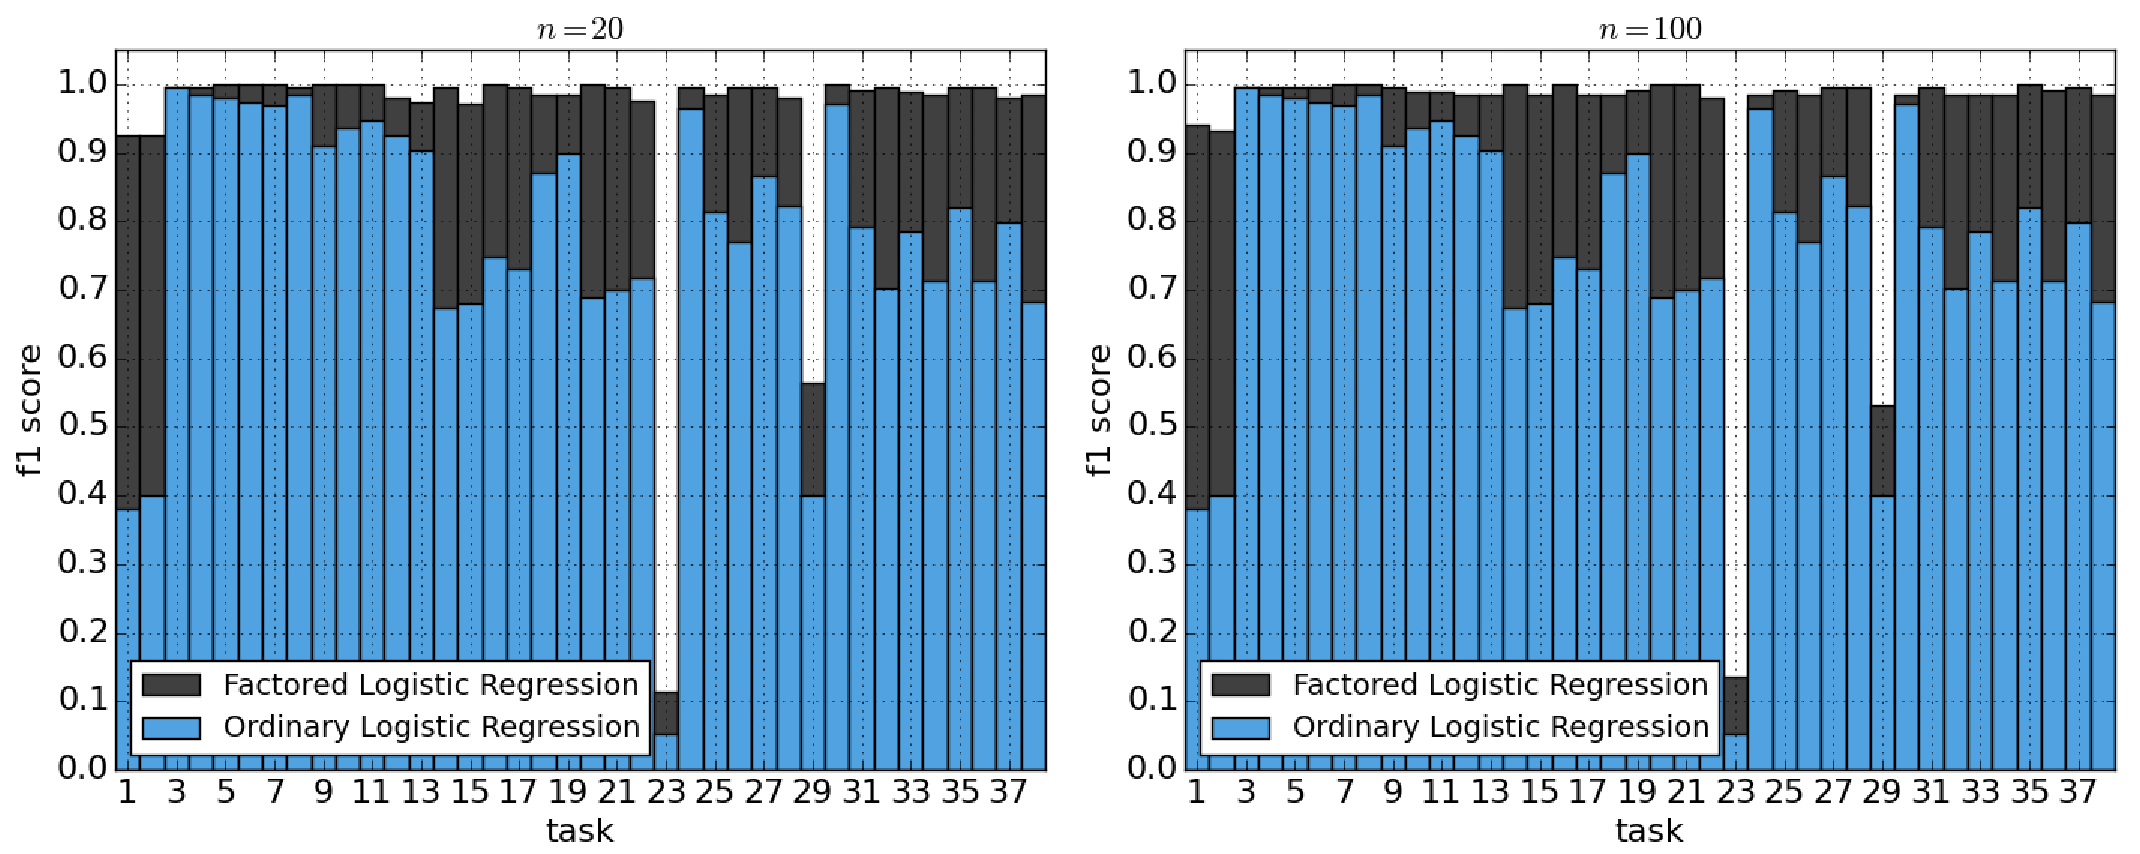
\includegraphics[width=1.00\textwidth]{figures/accuracies.pdf}
\end{centering}
\vspace{-0.5cm}
\caption{\textbf{Effect of bottleneck in a 38-task classificaton problem}
Depicts the f1 score for each of 38 class predictions (chance is  $2,6\%$)
sorted from lowest to highest.
Multinomial logistic regression operating in voxel space (\textit{blue bars})
was compared to 
SSFLogReg operating in $20$
(\textit{left plot}) and $100$ (\textit{right plot})
latent modes (\textit{grey bars}).
Autoencoder or rest data were not used for these analyses
($\lambda=1$).
Ordinary logistic regression yielded 77,7\% accuracy out of sample, while
SSFLogReg scored at 94,4\% ($n=20$) and 94,2\% ($n=100$).
Hence, compressing the voxel data into a component space for classification
achieves higher task separability.
}
\label{fig_dimred}
\end{figure}

We then quantified the impact of structure from rest data keeping
all model parameters constant
($n=20$, $\lambda=0.5$, $\ell_1=0.1$, $\ell_2=0.1$).
At the beginning of every epoch,
2000 task and 2000 rest maps were drawn with replacement
from same amounts of task maps but varying amounts of rest maps.
In frequently encountered data-scarce settings
($\approx{100}$ labeled samples),
but not in data-rich settings ($\approx{1000}$ labeled samples),
the repertoire of rest structure modulated model performance
(Figure \ref{fig_semisup}).

\begin{figure}
\begin{centering}
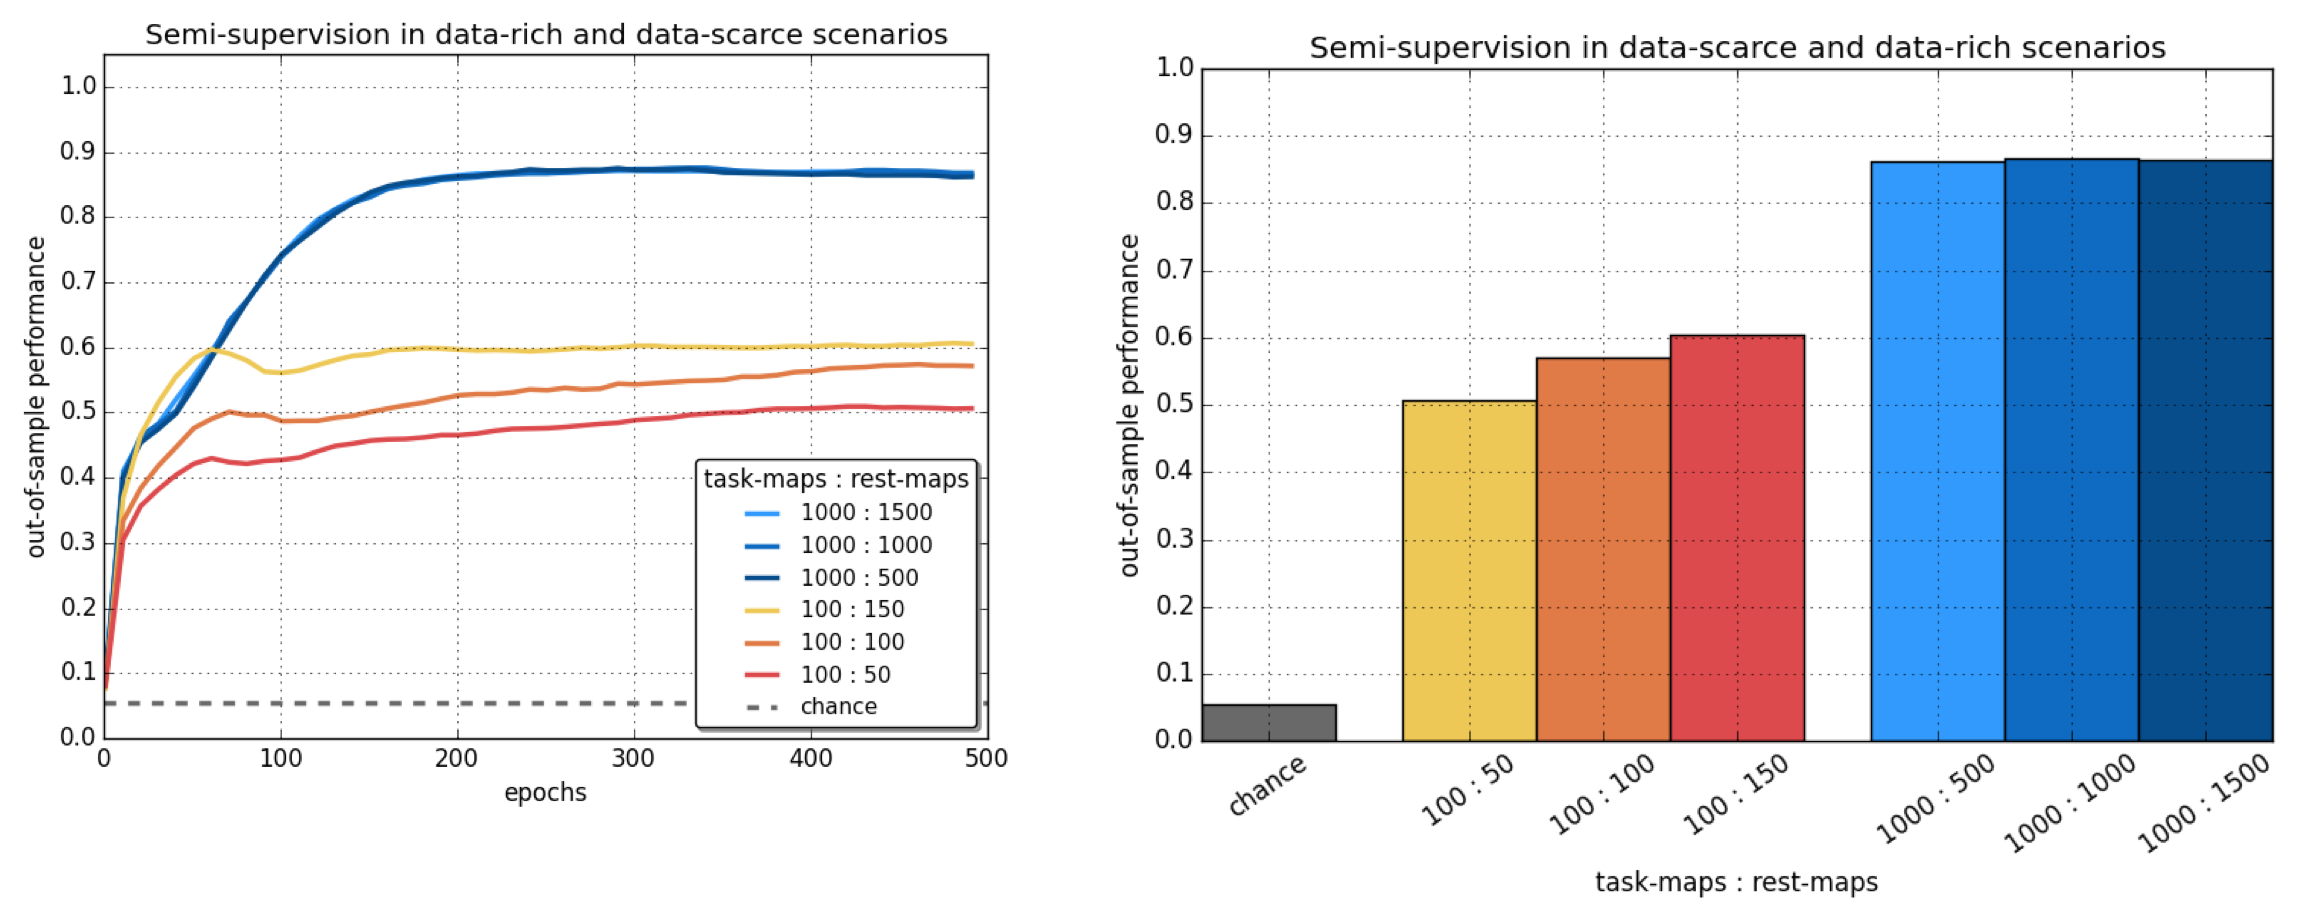
\includegraphics[width=1.00\textwidth]{figures/semisup_both.png}
\end{centering}
\vspace{-0.5cm}
\caption{\textbf{Effect of richness in rest data}
Gradient descent was performed on 2000 task and 2000 rest maps.
These were drawn with replacement from identical versus varying
quantities of task versus rest maps, at the begining of each epoch.
Chance is at 5,6\%.
}
\label{fig_semisup}
\end{figure}

\paragraph{Feature identification.}
We finally examined whether the models
were fit for purpose
(Figure \ref{fig_weights}).
%
To this end, we computed Pearson's correlation between the classifier weights
and the averaged neural activity map for each of the 18 tasks.
%
Ordinary logistic regression thus yielded a mean correlation
of $\rho=0.28$ across tasks.
%
For SSFLogReg ($\lambda=0.25, 0.5, 0.75, 1$),
a per-class-weight map was computed by matrix
multiplication of the two inner layers.
Feature identification performance thus ranged
between $\rho=0.35$ and $\rho=0.55$ for $n=5$,
between $\rho=0.59$ and $\rho=0.69$ for $n=20$, and
between $\rho=0.58$ and $\rho=0.69$ for $n=100$.
%
Consequently,
SSFLogReg puts higher absolute weights on relevant structure.
This reflects an increased signal-to-noise ratio, in part explained
by the more BOLD-typical local contiguity.
%
Conversely, SSFLogReg puts lower probability mass on irrelevant structure.
Despite lower interpretability of the results from
ordinary logistic regression, the
salt-and-pepper-like weight maps were sufficient for
good classification performance.
%
\begin{figure}
\begin{centering}
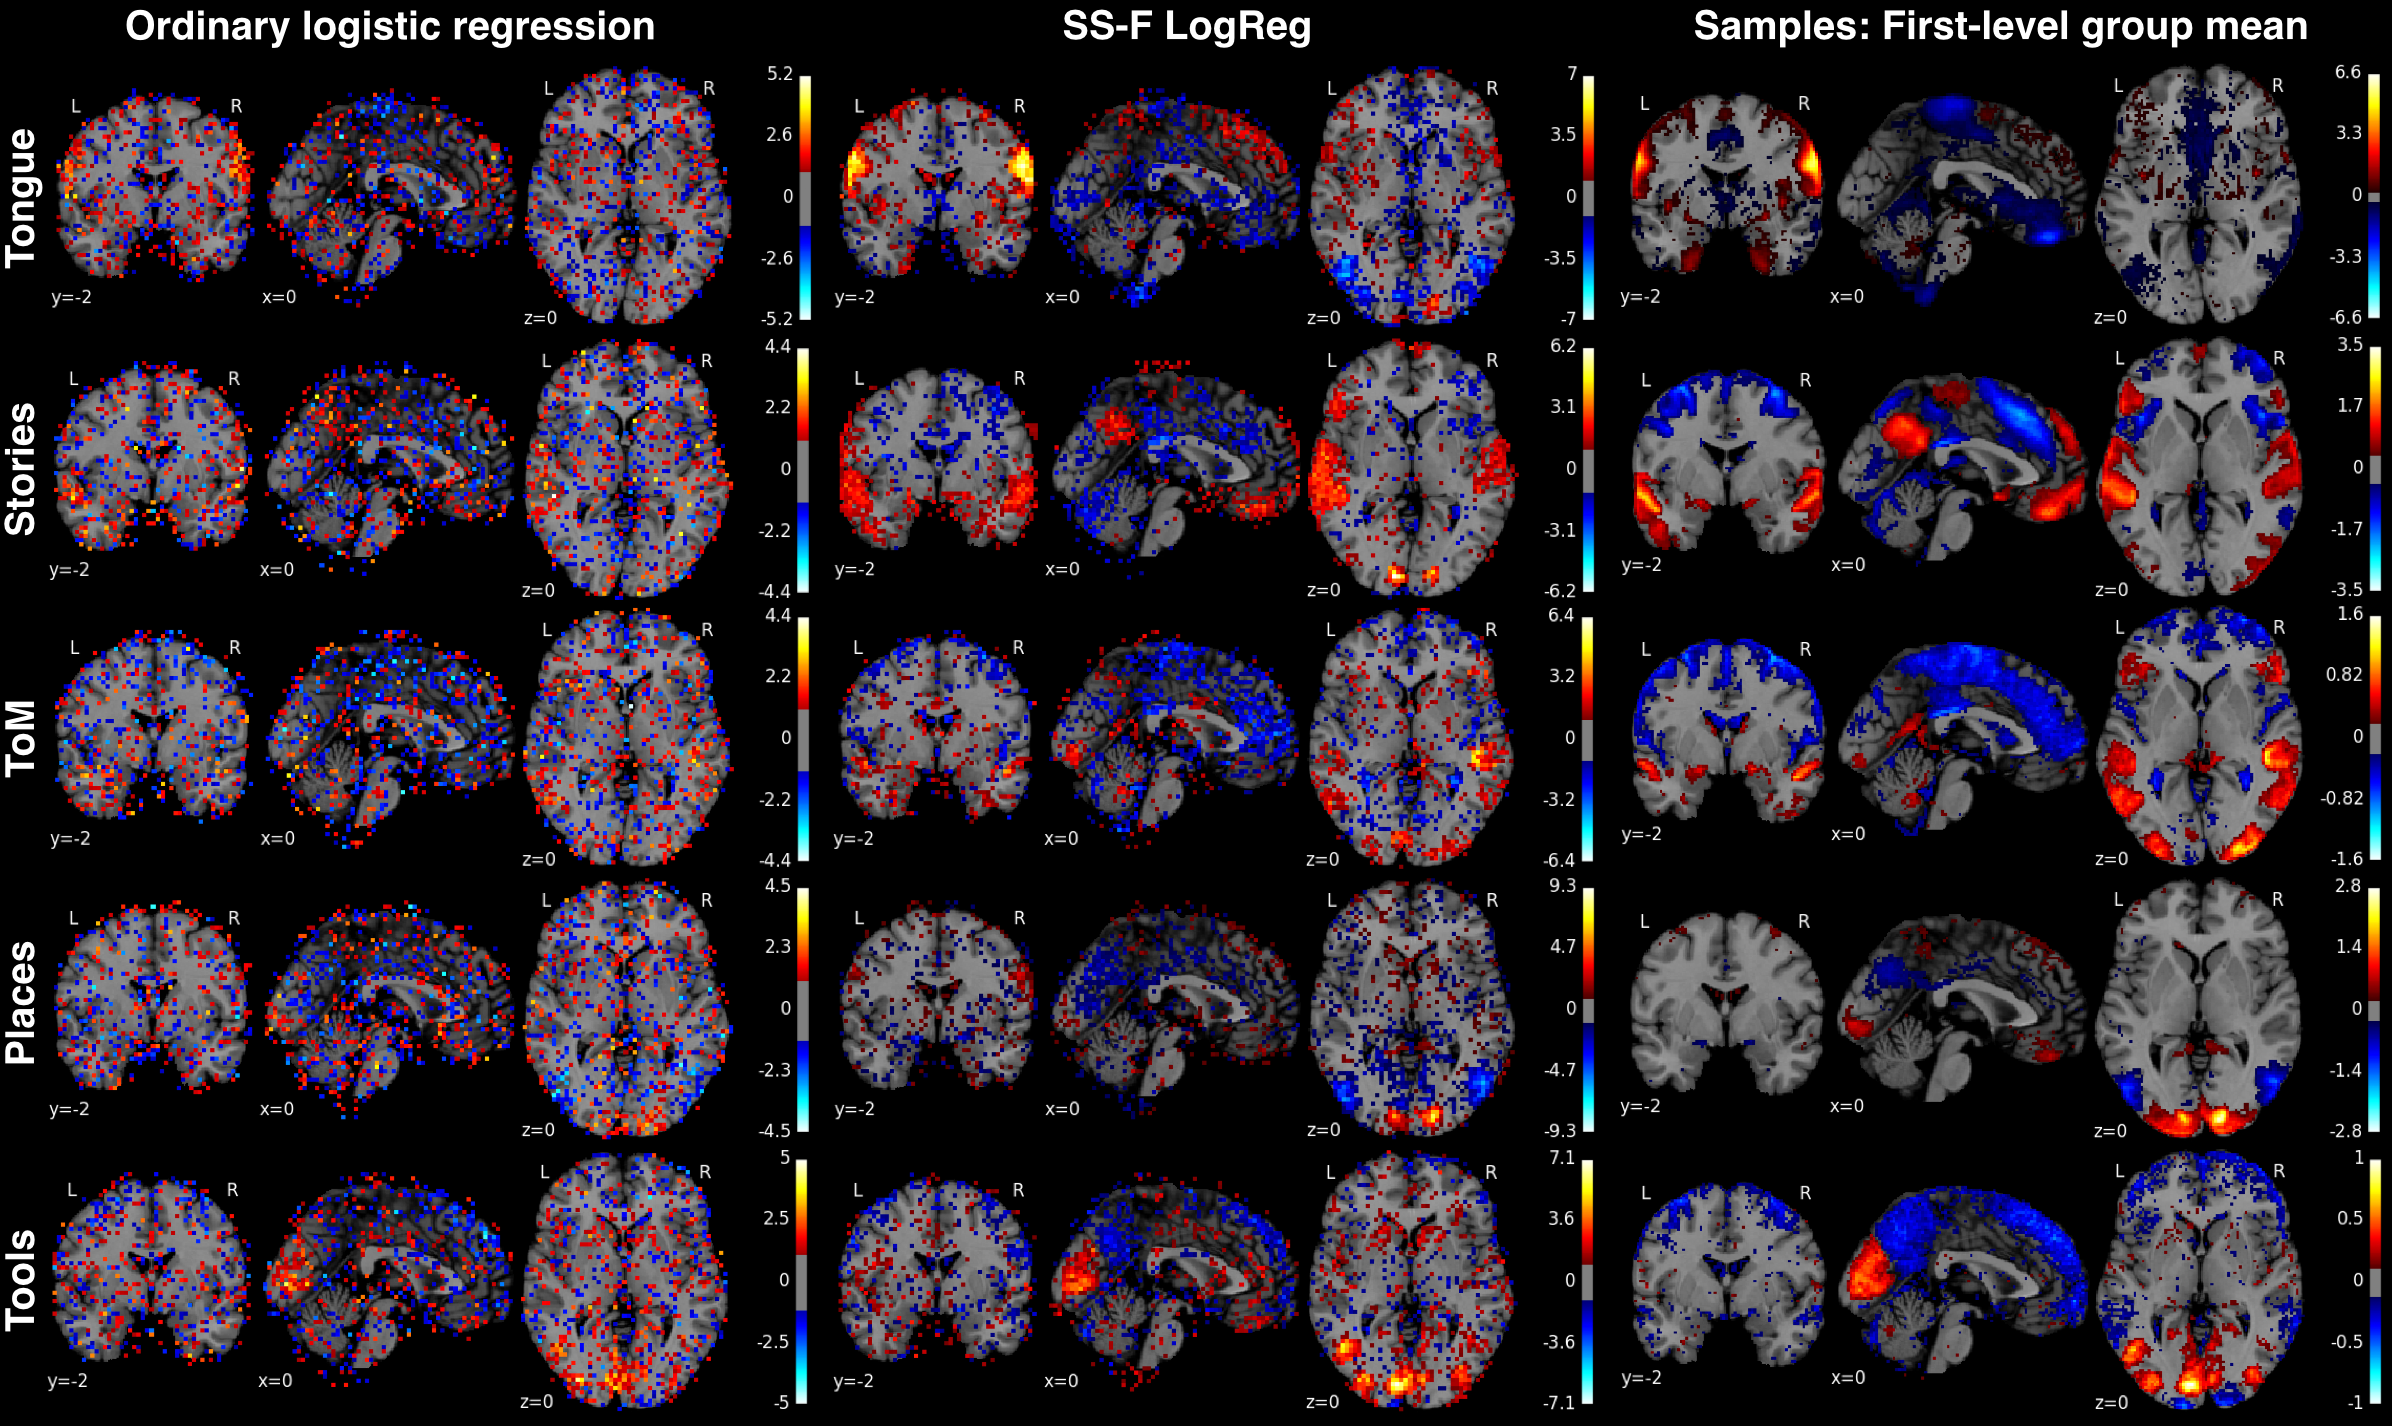
\includegraphics[width=0.98\textwidth]{figures/figure_weights_perc75.png}
\end{centering}
\vspace{-0.1cm}
\caption{\textbf{Classification weight maps}
The voxel predictors corresponding to 5 exemplary
(of 18 total) psychological tasks (\textit{rows})
from the HCP dataset \cite{barch2013}.
\textit{Left column:} multinomial logistic regression (same
implementation but without bottleneck or autoencoder),
\textit{middle column:} semi-supervised factored logistic regression
($n=20$ latent components, $\lambda=0.5$, $\ell_1=0.1$, $\ell_2=0.1$),
\textit{right column:} voxel-wise average across all samples of whole-brain
activity maps from each task.
Semi-supervised factored logistic regression
a) puts higher absolute weights on relevant structure,
b) lower ones on irrelevant structure,
and
c) yields BOLD-typical local contiguity (without enforcing a spatial prior).
All values are z-scored and thresholded at the $75^{th}$ percentile.
}
\label{fig_weights}
\end{figure}
%
Hence, SSFLogReg yielded class weights 
that were much more similar to features of the respective training samples
for all choices of $n$ and $\lambda$.
SSFLogReg therefore
captures genuine properties of neural activity patterns,
rather than participant- or study-specific artefacts.

\paragraph{Miscellaneous observations.}
For the sake of completeness,
we informally report modifications of the statistical model
that did not improve generalization performance.
%
Introducing stochasticity into model learning by 
$a)$ input corruption of $\mathbf{X_{task}}$ or
$b)$ drop-out at the bottleneck $\mathbf{W_0}$ using binomial
distributions ($p=0.1, 0.3, 0.5$) deteriorated model performance
in all scenarios.
%
Adding $c)$ rectified linear units (ReLU) to $\mathbf{W_0}$ or
other commonly used nonlinearities ($d)$ sigmoid, $e)$ softplus,
$f)$ hyperbolic tangent) all led to decreased classification accuracies,
probably due to sample size limits.
%
Further, $g)$ ``pretraining'' of the bottleneck $\mathbf{W_0}$
(i.e., non-random initialization) by 
either corresponding SPCA or ICA loadings did not exhibit improved accuracies,
neither did $h)$ autoencoder pretraining.
%
Moreover,
introducing an additional $i)$ overcomplete layer (100 units)
after the bottleneck was not advantageous.
%
Finally, imposing either $j)$ only $\ell_1$ or 
$k)$ only $\ell_2$ penalty terms
was disadvantageous in all tested cases,
which favored ElasticNet regularization chosen in the above analyses.

\section{Discussion and Conclusion}
% Conceptual recap+gain of current paper
Using the flexibility of factored models,
we learn the low-dimensional representation from high-dimensional
voxel brain space that is most important for
prediction of cognitive task sets.
%
From a machine-learning perspective,
factorization of the logistic regression weights
can be viewed as transforming a
``multi-class classification problem''
into a ``multi-task learning problem''.
%
The higher generalization accuracy and feature recovery, comparing to
ordinary logistic regression, hold potential
for adoption in various neuroimaging analyses.
Besides increased performance, these models are more interpretable by
automatically learning a mapping to and from a brain-network space.
%
This domain-specific learning algorithm
encourages departure from the artificial and statistically
less attractive voxel space.
Neurobiologically,
brain activity underlying defined mental operations
can be explained by linear combinations of the main activity
patterns.
%
That is,
fMRI data probably concentrate near
a low-dimensional manifold of
characteristic brain network combinations.
Extracting fundamental building blocks of brain organization might
facilitate the quest for the cognitive primitives of
human thought.
%
We hope that these first steps stimulate development towards
powerful semi-supervised representation extraction
in systems neuroscience.

% grand perspective
In the future, automatic reduction of brain maps to
their neurobiological essence
may leverage data-intense neuroimaging investigations.
Initiatives for data collection are rapidly increasing
in neuroscience \cite{poldrack2014data}.
These promise structured integration
of neuroscientific knowledge accumulating
in databases.
Tractability by
condensed feature representations can avoid the ill-posed problem of
learning the full distribution of activity patterns.
%
This is not only relevant to the 
multi-class challenges spanning the human cognitive space
\cite{schwartz2013mapping}
but also the
multi-modal combination with
high-resolution 3D models of brain anatomy \cite{amunts2013bigbrain}
and
high-throughput genomics \cite{need2010gwas}.
%
The biggest socioeconomic potential may
lie in across-hospital clinical studies that
predict disease trajectories and drug responses
in psychiatric/neurological populations
\cite{frackowiak2015future, gustav2011cost}.

\paragraph{Acknowledgment}
{\small
Data were provided by the Human Connectome Project.
% The study was supported by the German National Academic Foundation (D.B.).
}

\small
\bibliographystyle{splncs03}
\bibliography{nips_refs}

\newpage
\section{Appendix}
%
\paragraph{Data.}
As the currently biggest openly-accessible reference dataset,
we chose the Human Connectome Project (HCP) resources
\cite{barch2013}.
Neuroimaging task data with labels of ongoing cognitive processes
were drawn from 500 unrelated,
healthy HCP participants.
18 HCP tasks 
were selected that are known to elicit reliable neural activity
across participants.
The task paradigms include
1) working memory/cognitive control processing, 2)
incentive processing, 3) visual and somatosensory-motor processing,
4) language processing (semantic and phonological processing),
5) social cognition, 6) relational processing, and 7) emotional
processing. All data were acquired on the same Siemens Skyra 3T scanner.
Whole-brain EPI acquisitions were acquired with a
32 channel head coil (TR=720ms, TE=33.1ms, flip angle=52°, BW=2290Hz/Px,
in-plane FOV=$280\textrm{mm}\times180\textrm{mm}$, 72 slices, 2.0mm 
isotropic voxels).
The ``minimally preprocessed'' pipeline includes
gradient unwarping, motion correction, fieldmap-based EPI distortion
correction, brain-boundary-based registration of EPI to structural
T1-weighted scans, nonlinear (FNIRT) registration into MNI space,
and grand-mean intensity normalization. Activity maps were spatially
smoothed with a Gaussian kernel of 4mm (FWHM). A GLM was
implemented by FILM from the FSL suite with model regressors from convolution
with a “canonical” hemodynamic response function and from temporal derivatives.
HCP tasks were conceived to modulate activity
in a maximum of different brain regions and neural systems. Indeed, at
least 70\% of the participants showed consistent brain activity in
contrasts from the task battery, which certifies excellent
activity patterns covering extended parts of the brain \cite{barch2013}.
%
In sum, the HCP task data incorporated 8650 first-level activity maps
from 18 diverse paradigms administered to 498 participants (2 removed
due to incomplete data).
All maps were resampled to a common 60x72x60 space of
3mm isotropic voxels and gray-matter masked (at least 10\% tissue
probability).
The supservised analyses were based on labeled HCP task maps with
79,941 voxels of interest representing z-values in gray matter.

These labeled data were complemented by unlabeled activity maps
from HCP acquisitions of unconstrained resting-state activity
\cite{smith2013resting}.
These reflect brain activity in the absence of controlled thought.
In line with the goal of the present study, acquisition of these data was
specifically aimed at the study of task-rest correspondence.
From each participant, we included two
time-series for left and right phase encoding
with 1,200 maps of multiband, gradient-echo planar imaging acquired
during a period of 15min (TR=720 ms, TE=33.1 ms, flip angle=52°,
FOV=$280\textrm{mm}\times180\textrm{mm}$, and 2.0mm isotropic voxels). 
Besides run duration,
the task acquisitions were identical to the resting-state fMRI acquisitions
for maximal compatibility between task and rest data.
We here drew on ``minimally preprocessed'' rest data
from 200 randomly selected healthy, unrelated participants.
PCA was applied to each set of 1,200 rest maps for
denoising by keeping only the 20 main modes of
variation.
In sum, the HCP rest data concatenated
8000 unlabeled, noise-cleaned rest maps with
40 brain maps from each of 200 randomly selected participants.

We were further interested in the utility of the
optimized low-rank projection
in one task dataset for dimensionality reduction in another task dataset.
To this end, the HCP-derived network decompositions were used as preliminary
step in the classification problem of another large sample.
The ARCHI dataset \cite{pinel07} provides activity maps from
diverse experimental tasks, including auditory and visual perception, motor action,
reading, language comprehension and mental calculation.
81 right-handed healthy participants
(3 not included in present analyses due to incomplete data)
without psychiatric or
neurological history participated in four fMRI sessions acquired under
different experimental paradigms.
The functional maps were warped into
the MNI space and resampled to isotropic 3mm resolution.
Whole-brain EPI data were acquired with the same Siemens Trio with a 32
channel head coil (TR=2400ms, TE=30ms, flip angle=60°, in-plane
FOV=$192\textrm{mm}\times192\textrm{mm}$, 40 slices, 3.0mm isotropic voxels).
Standard preprocessing was performed with Nipype \cite{gorgo11}, including
slice timing, motion correction, alignment, and spatial normalization.
Activity maps were spatially smoothed by
a Gaussian kernel of 5mm (FWHM).
Analogous to HCP data, the second task dataset incorporated 1404
labeled, grey-matter masked, and z-scored activity maps
from 18 diverse tasks acquired in 78 participants.

\end{document}
